\section{Pantallas de la aplicación}

\subsection{Pantalla de inicio de sesión}
%se pone el nombre de la pantalla que se reportará

\subsection{Descripción}
%Descripción amplia de las funciones de la pantalla incluyendo la descripción de todos los botones y las validaciones con las que cuenta
En esta pantalla el usuario puede autenticarse a la aplicación para acceder a su panel de correspondencia. Contiene un campo de texto para introducir su correo con el cual se autenticará, otro campo de texto para introducir la contraseña y un botón de "Iniciar sesión" para que la aplicación haga la validación de los datos introducidos y de acceso al usuario.

%imagen de la pantalla
	\begin{figure}[htbp!]
		\centering
			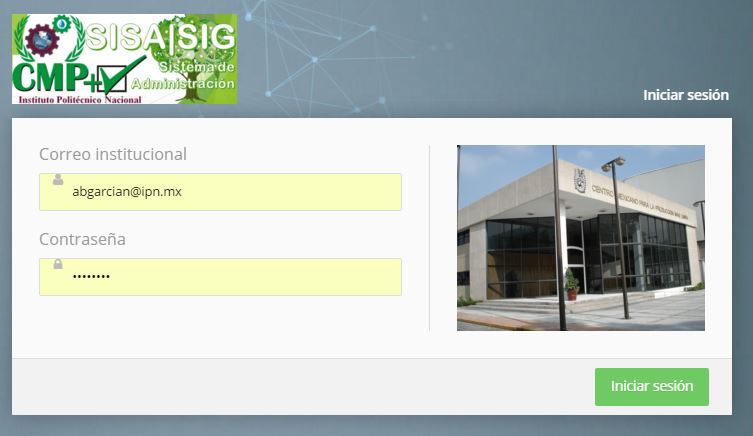
\includegraphics[width=0.8\textwidth]{Pantallas/iniciodesesion}
		\caption{Pantalla de inicio de sesión.}
	\end{figure}

\subsection{Funcionamiento}
%Descripción del funcionamiento de la pantalla
Se describe el proceso o procesos que se realizan en está pantalla. (puedes usar item)
\subsection{Problemas que resuelve}
	\begin{itemize}
		\item Que la Kenia pueda controlar mejor la correspondencia.
		\item Que lulú esté contenta.
	\end{itemize}

\subsection{Pantallas relacionadas}
Está pantalla se relaciona con las siguientes pantallas:
	\begin{itemize}
		\item 3.2 Pantalla de panel principal del usuario.
	\end{itemize}